\documentclass[tikz]{standalone}
\usepackage{tikz,amsmath}
\usetikzlibrary{shapes}

%\pgfmathdeclarefunction{f}{1}{%
%\begingroup
% \pgfmathparse{1-#1*#1}
% \pgfmath@smuggleone\pgfmathresult%
%\endgroup}

\begin{document}
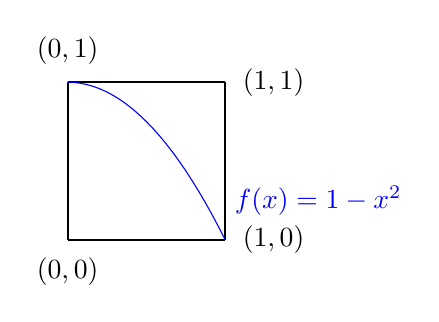
\begin{tikzpicture}[scale=2]
    \draw [thick, step=1cm] (0,0) grid (1,1);
    \node [right=.1cm] at (1,0) {$(1,0)$};
    \node [right=.1cm] at (1,1) {$(1,1)$};
    \node [below=.1cm] at (0,0) {$(0,0)$};
    \node [above=.1cm] at (0,1) {$(0,1)$};

    \draw[domain=0:1, color=blue] plot (\x, {1- (\x)^2}) node[above = .5cm, right, color=blue] {$f(x)=1-x^2$};

%\draw[domain=-1:1, color='blue'] plot (\x,{f(\x)})
\end{tikzpicture}
\end{document}
